\documentclass[]{htwg-report}


\addbibresource{./bib/library.bib}

\hyphenation{Sca-la-la}
\hyphenation{Sca-la-Ka-ta}
\hyphenation{Sca-la-la-Ka-ta}



\begin{document}

%% Use Roman numerals for the page numbers of the title pages and table of
%% contents.
\frontmatter

%% 'reporttype' add background elements to the cover / front page
%% possible values are:
%% bachelor	--> B S C
%% master	--> M S C
%% other		--> none
\reporttype{bachelor}

\reporttypetext{Bachelor Thesis}

\title[A DSL and web-based Interpreter for Music Notation]{A Domain-Specific Language and web-based Interpreter for Music Notation}

\author{Markus Funke}
\studentnumber{291992}
\studentemail{markus.funke@htwg-konstanz.de}

\doclocation{Konstanz}
\docdate{31st July 2018}

\makecover[]
%          
%% Include an optional title page.
\input{title}

\chapter*{}
\begingroup
{\makeatletter

\begin{figure}[h]
\centering
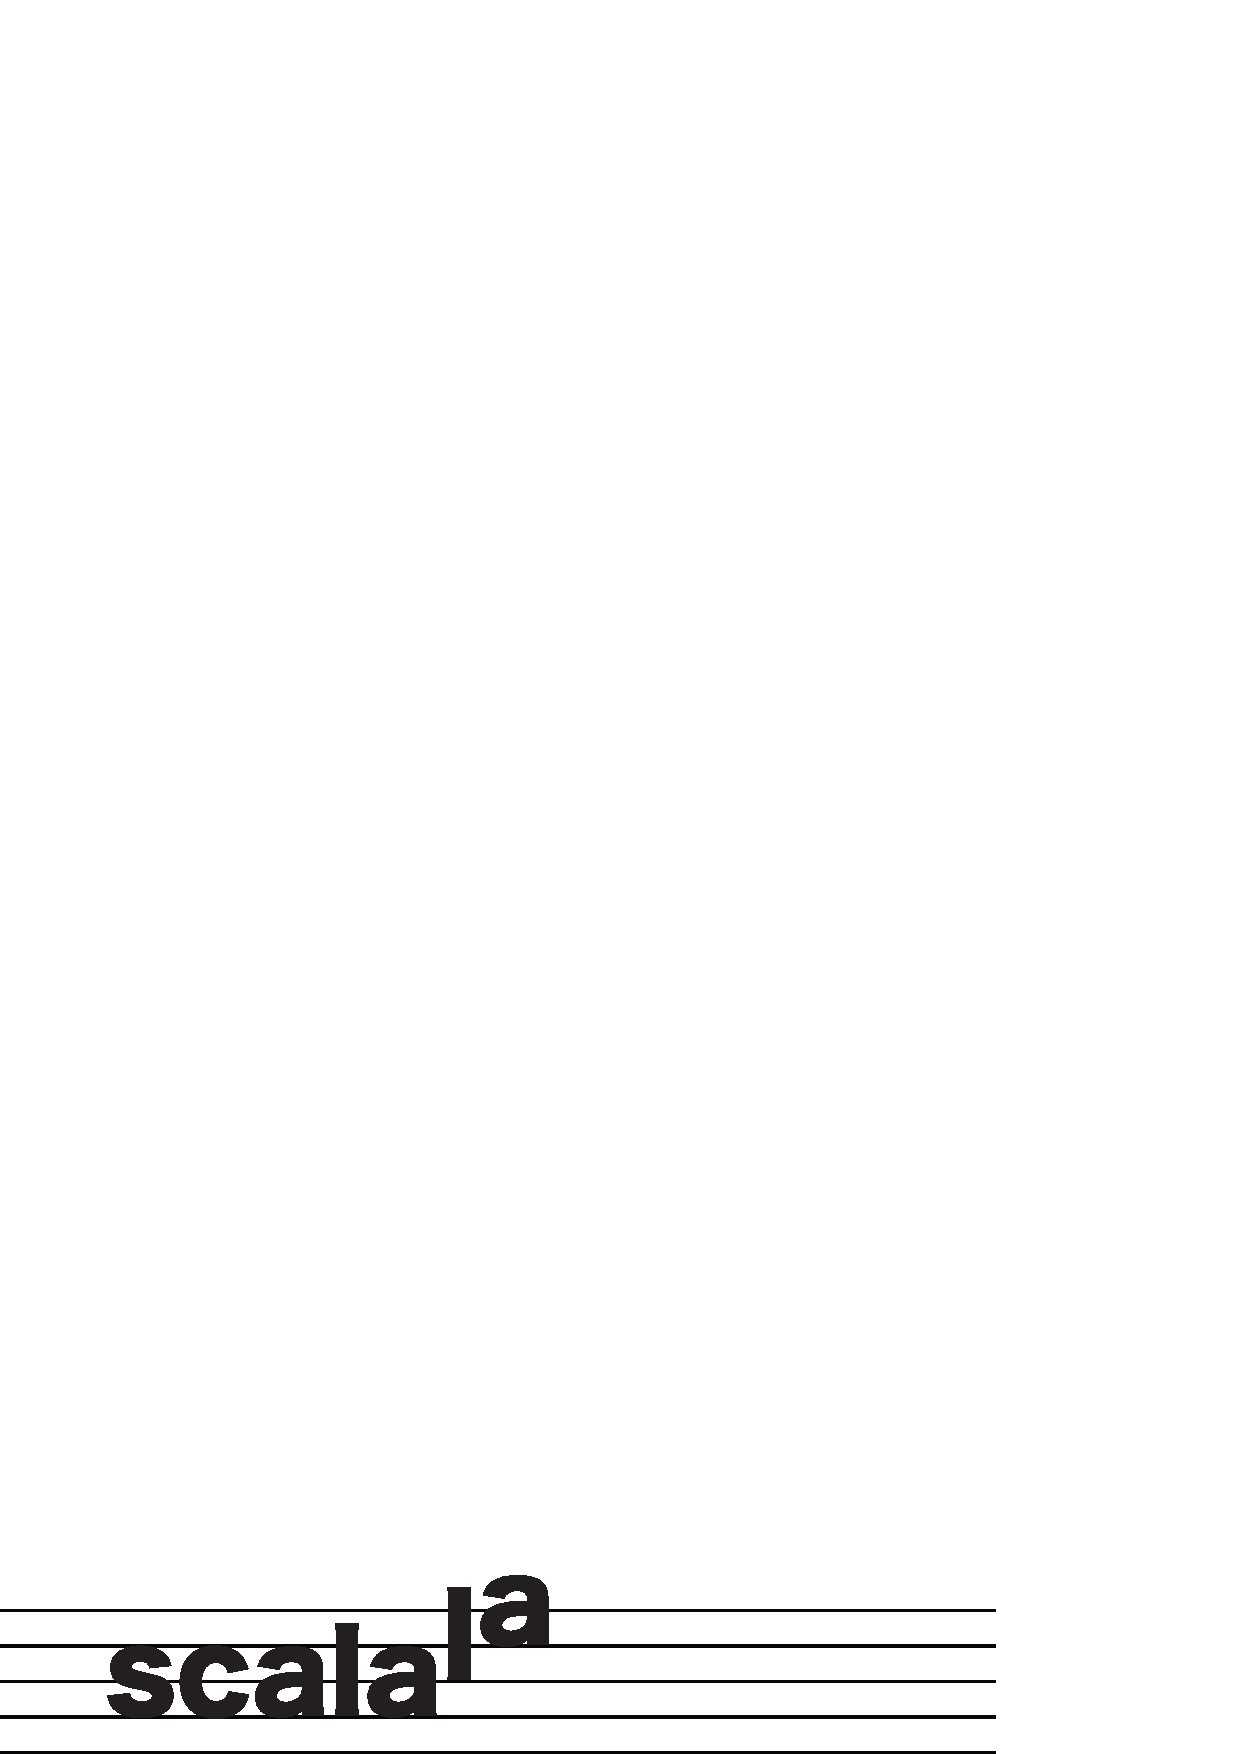
\includegraphics[scale=0.7]{scalala}
\end{figure}

\bigskip
\bigskip

\begin{center}
\Huge\textbf{A Domain-Specific Language \newline and web-based Interpreter \newline for Music Notation}
\newline
\newline
\LARGE\textbf{\@author}
\end{center}

\makeatother}
\endgroup


\chapter*{Ehrenwörtliche Erklärung}
\setheader{Ehrenwörtliche Erklärung}

\begingroup
{\makeatletter
Hiermit erkläre ich, \@author, geboren am 14.05.1989 in Landsberg am Lech,



\renewcommand*{\arraystretch}{1.5}
\rowcolors{2}{white}{white}
\begin{tabular}{p{50pt}p{320pt}}
         & \\
    (1) & dass ich meine Bachelorarbeit mit dem Titel: \newline \newline  
\textbf{"A Domain-Specific Language and web-based Interpreter for Music Notation"} \newline \newline in der Fakultät Informatik unter Anleitung von Professor Dr. Marko Boger selbständig und ohne fremde Hilfe angefertigt habe und keine anderen als die angeführten Hilfen benutzt habe; \\ \\
    (2) & dass ich die Übernahme wörtlicher Zitate, von Tabellen, Zeichnungen, Bildern und Programmen aus der Literatur oder anderen Quellen (Internet) sowie die Verwendung der Gedanken anderer Autoren an den entsprechenden Stellen innerhalb der Arbeit gekennzeichnet habe. \\ \\
    (3) & dass die eingereichten Abgabe-Exemplare in Papierform und im PDF-Format vollständig übereinstimmen. \newline \newline
\end{tabular}

Ich bin mir bewusst, dass eine falsche Erklärung rechtliche Folgen haben wird.


\begin{tabular}{lp{200pt}l}
  & & \\ \\
  Konstanz, 31.07.2018 & & \@author 
\end{tabular}


\makeatother}
\endgroup

\chapter*{Abstract}
\setheader{Abstract}

Internal Domain-Specific Languages (DSLs) are typically well known by engineers and developers in form of APIs. External DSLs are used by business employees–the domain experts–to modify enterprise software without having to rely on the developers. However, both are experts in their own language.
The aim of this study is to create a music-notation language for both, technical and non-technical users. Through the usage of the DSL, basic concepts of programming languages as well as simple music notation can be taught.
Already conducted research has shown how to create music with written language or how sheet music can be created programmatically, but both of them are limited to people with an understanding of physical-modelling-synthesis or knowledge of programming.
This thesis investigates the capabilities to write music notation, or rather, to program music without programming expertise.
It used the cardinality of external DSLs in Scala to design a user-friendly language.
Beyond that, the generation and the playback of sound and written music, as well as the whole pipeline between the language interpreter and the web-based interface with Scala.js, was implemented.
As a result, the thesis presents a holistic web application to explore the capabilities of the developed language and discuss the application of the language to teach programming novices.


\tableofcontents

%% Use Arabic numerals for the page numbers of the chapters.
\mainmatter


\chapter{Introduction}
\label{INTRO}
Teaching programming has become increasingly important over the last years. Moreover, teaching children how to program at school is at least equally important as teaching them at university. As a result, programming languages and applications need to be devised for an educational background. The following chapter gives an introduction to this subject and will explain why and how a domain-specific language can help teach programming. The methodology elaborates how to design a programming language and how to integrate this approach into a holistic solution. At the end of this section, the structure of this research is outlined.

\section{General}
\label{INTRO_GEN}
In Schnabel's research 2011 he said:
\begin{quote}
"only through giving students deep computer science (CS) knowledge can we expect to have a new generation that can create—not just consume—the next wave of computing innovations."\cite{Schnabel2011}
\end{quote}
However, to create this new generation, it is necessary to find new approaches to teach programming. One method is to combine gamification with programming or use hardware with programming. Section \ref{LIT_PROJ} shows related projects for each approach. Soloway et al. suggest to pack expert knowledge into the natural language.\cite{Soloway1982} Domain-specific languages (DSLs) offers this opportunity by creating a language style, which has a natural feel. However, teaching programming does not depend solely on the language; just as significant are the findings of the written program.\cite{Kahn1995} As mentioned above, one approach is to add other stimuli or charms. Adding music or sound to the learning procedure could increase the learning curve—for novices as well as children.

\section{Precedence of DSLs and Sound Generation}
\label{INTRO_PRECE}
DSLs are not a new technology and can be traced back to Ross, 1978.\cite{Ross1978} Usually, DSLs are a common way to offer developers a simple mechanism to interwork with higher complex software or give non-developers access to software projects to manipulate them. Many studies discuss the advantages of DSLs. Hofer et al. formulated that "simple interpreters can be quickly derived and implemented" and "it is easy to extend the DSL".\cite{Hofer2011} Fowler also names two reasons why developers should be interested in DSLs; they "improve programmer’s productivity" and they make program parts "easier to understand".\cite[p. xxi]{Fowler2010} This circumstance makes it evident that DSLs are an excellent approach to teach novices programming, regardless, the most notable disadvantage of DSLs are their complexity in development.\cite{Mernik2005}

The combination of programming and sound generation is not a new approach. The project \textit{Sonic Pi}\footnote{Sonic Pi - \url{http://sonic-pi.net}} provides a solution which focuses on sound generation through text description and offers an interactive environment.\cite{Aaron2013} The system is based on physical-modelling-synthesis, which means that user should have a minimum knowledge of classical sound synthesising techniques like wave amplitudes. Therefore, this approach adds a further knowledge-domain to the programming and music-domain. A more accessible approach is desirable.

\section{Combining Software and Music}
\label{INTRO_SOFT}
The purpose of this study is to describe and examine an approach to design a programming language for programming novices which is simple to read, understand and learn. The objective of the language is to teach the primary and elementary programming concepts like variable declaration, expressions, arithmetic or method invocation. This means that the language offers a suitable balance between the proximity to natural language and real computer science languages. Scala is used as global-purpose language (GPL) to develop the DSL, especially the parser and the corresponding interpreter. This work concentrates on the implementation of external DSLs, but discusses these in relation to internal DSLs and compares them. The DSL itself is not a Turing complete language by design and serves only one purpose: to create music through programming notes. The sound, or, more precisely, the music, which is a result of the corresponding DSL, is generated by a application written in Scala.

To provide a holistic approach, the user-interface is implemented as a web-based editor. The intention is to write and explore the DSL in a simple to use web-browser application, with the focus to provide fast feedback like syntax highlighting, as well as error feedback and the possibility to playback the written music. This web-application is also developed with Scala. The individual web components such as the editor, the music playback and the user interaction are written with the assistance of Scala.js.

\section{Objectives and Methodology}
\label{INTRO_METHOD}
This thesis is organised as follows: Chapter \ref{THEO} describes and provides the necessary theoretical knowledge and the primary intention. It describes DSLs in general, compares internal with external DSLs and shows how Scala acts as the center point of the project. Furthermore, MIDI as sound-medium is explained. Scala.js is identified as the central component for the web-based user-interface. Afterwards, chapter \ref{LIT} presents ongoing research projects and existing research resources in order to establish the state-of-the-art in the area of teaching programming, DSL development and sound generation by code. The methodology in chapter \ref{IMPL} firstly explains the technical implementation and illustrates the architecture. Secondly, the implementation is broken down into two parts. The first part discusses the DSL concept and implementation through Scala parser combinators in particular. The second part comprises the web-application, which serves as the client-server model for the holistic application. Beyond that, the client and the server make use of additional libraries such as multiple Scala.js façades, which are built as independent projects. In chapter \ref{RESULTS} the entire application is viewed at large. The inclusion of various DSL script examples and a minor case study serve as a basis for analysis. Finally, chapter \ref{DISCUSSION} provides a brief discussion of the results and gives a conclusion.




\chapter{Theoretical Principles}
\label{THEO}
The following chapter describes the necessary theoretical knowledge to understand the research process and development. Close attention is paid to DSLs in general and the difference between internal and external DSLs. Furthermore, the programming language Scala is analysed and is viewed from the DSL implementation perspective. With an introduction to Scala.js, the possibilities and limits of the Scala-to-JavaScript code compiler are illustrated. To provide a better comprehension of the design and development decisions, the MIDI system is introduced and discussed.

\section{Domain Specific Languages}
\label{THEO_DSL}
Almost all programming languages are defined as a Turing complete and a general-purpose language (GPL). However, most programming languages are also designed for a specific purpose. For example, the Java design goal is to develop "highly robust applications on multiple platforms in heterogeneous, distributed networks".\cite{Gosling1996} The Prolog language is associated with artificial intelligence.\cite{Bowen1981} PHP is described as a language which is designed for "web development".\cite{ThePHPGroup} However, these design goals indicate that these languages are more domain-specific than general-purpose languages.\cite{Mernik2005} It is evident that something is more comfortable to use when the instrument is developed for a specific context. For example, PHP opens web development to a larger group of developers as Prolog (despite the opportunity to build web applications in Prolog), since the PHP language and its syntax are closer to this domain—the web-development domain. This is the exact starting point for DSLs—abstract a specific domain problem and make it accessible for the domain experts.

Apart from the fact that any GPL is in a particular way a DSL, in almost all cases a DSL is provided through a GPL. The consequence of this principle is that the DSL has to be implemented with the GPL and has to extend it, to provide a user-friendly language on top.\cite{Ghosh2010} Ghosh and other authors define this concept as "metalinguistic abstraction"\cite[p. 15]{Ghosh2010}. The next two subsections describe two ways to implement a DSL through a GPL, the internal and the external.

\subsection{Internal DSL}
\label{THEO_DSL_INTERN}
Internal (also called embedded) DSLs are often described with, or compared to an application programming interface (API).\cite{Mernik2005, Ghosh2010, Riti2018} Since an internal DSL is a direct subset of the GPL, the syntax must be the same as the GPL. Despite this condition, an internal DSL is well suitable to create a \textit{fluent interface}. The terminology "fluent" is described by Fowler.\cite{Fowler2010} The term means that the DSL is closely developed to the natural language and offers a syntax where the expressions and statements of the DSL are readable like human language. Underneath, the DSL is a concatenation of function calls. In section \ref{THEO_SCALA} the Scala GPL is introduced and it is discussed why the Scala language is a perfect fit for defining internal DSLs.

In the following example, a pseudo-GPL is illustrated. The pseudo-GPL is defined as function calls which are invoked by using \texttt{->}. Consider the domain in which the DSL is applied for: the administration of a shopping market. The domain administrator wants to be able to set product prices and order new products. The traditional GPL approach is to define objects and functions with parameters and take advantage of method chaining.

\begin{center}
\texttt{new Product('coffee')->makeOffer(10)->until(2018-05-14)}
\end{center}

The pseudo code above creates a new object of the type \texttt{product} with the name \texttt{coffee} and calls the class method \texttt{makeOffer} with the price \texttt{10} as argument. Through method chaining a new object of the type \texttt{offer} is returned which provides the function \texttt{until} to set an end date for the offer. This syntax is familiar to developers and programmers. In the next step, the GPL specific elements, like the arrow \texttt{->} and parentheses are highlighted and subsequently eliminated.

\begin{center}
\texttt{ \textbf{new} Product\textbf{('}coffee\textbf{')->}createOffer\textbf{(}10\textbf{)->}until\textbf{(}2018-05-14\textbf{)}}
\end{center}

\begin{center}
\texttt{Product coffee createOffer 10 until 2018-05-14}
\end{center}

An almost fluent sentence was created which is close to the natural language. The next listing will add additional words to complete the statement to an approximately natural sentence.

\begin{center}
\texttt{for the product coffee create an offer of 10 EUR until 2018-05-14}
\end{center}

As in the listings above illustrated, it is possible to create a fluent API just with tools of the GPL. Furthermore, internal DSLs can be classified according to their relation to the host GPL.

\begin{figure}[h]
\caption{GPL Extension and Reduction.\cite{Fleming2015}}
\label{IMG_DSL-RED-EXT}
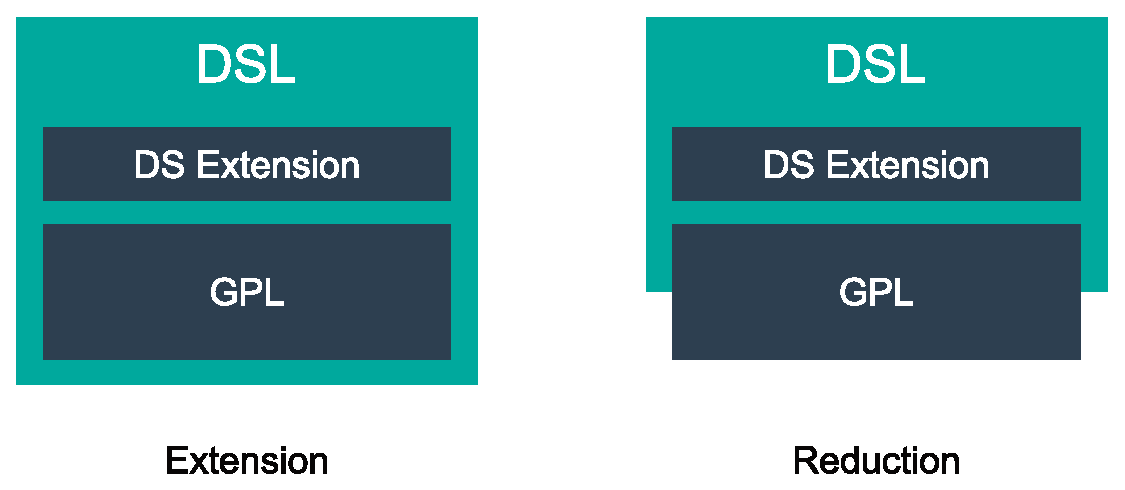
\includegraphics[scale=0.5]{dsl_extension_reduction}
\end{figure}

Figure \ref{IMG_DSL-RED-EXT} shows two classes of internal DSLs. The left side presents the GPL extension. This means that the developer provides the DSL user with the entire GPL functionality and on top of it—the DSL functionality. The right site represents the reduction of the GPL. The advantage of this approach is that the DSL is just an extract of the GPL and reduces its complexity, which, in turn, significantly increases simplicity.\cite{Schmitt2014}

\subsection{External DSL}
\label{THEO_DSL_EXTERN}
In comparison to the internal approach, an external DSL has no restrictions in defining the language since it is completely decoupled from the GPL. Therefore, the developed language can be very close to the language which is used in the target domain. However, the negative aspect of this total flexibility is the effort required in its implementation. Due to the fact that external DSLs are not coupled to the GPL syntax, the parser and interpreter have to be developed additionally. External DSLs are further discussed in chapter \ref{IMPL_SCALALA}.


\section{Scala}
\label{THEO_SCALA}
Scala offers useful tools, to define and develop DSLs. This is because of the circumstance that Scala combines two programming paradigms: object orientated and functional programming. Beyond that, the Scala GPL offers support for function calls without the dot notation or parentheses. The example given in section \ref{THEO_DSL_INTERN} is therefore already valid Scala code. This enables a clean code solution that is also simple to maintain.\cite{Riti2018} Chapter \ref{IMPL_SCALALA} presents essential concepts of Scala. For example: traits, pattern matching, case classes and higher-order functions and why these are necessary and useful for developing DSLs.

\section{Scala.js}
\label{THEO_SCALAJS}
To embrace the developed DSL in a holistic approach, a web-interface was developed. The whole client-application is written in Scala.js. Scala.js is a compiler that translates Scala code to equivalent JavaScript code; like its counterpart TypeScript. It offers an easy to use approach to write familiar Scala code with all its benefits like type safety, immutability, collections and pattern matching. See listings \ref{LS_NATIVE_JS} and \ref{LS_SCALAJS} to compare native JavaScript classes with Scala.js classes.\cite{ScJsDoc}

\begin{lstlisting}[caption={Native JavaScript Class Example}, label=LS_NATIVE_JS]
var Person = function(firstName, lastName) {
  this.firstName = firstName;
  this.lastName = lastName;
};

Person.prototype.fullName = function() {
  return this.firstName + " " + this.lastName;
};
\end{lstlisting}


\begin{lstlisting}[caption={Scala.js Class Example}, label=LS_SCALAJS]
class Person(val firstName: String, val lastName: String) {
  def fullName(): String =
    s"$firstName $lastName"
}
\end{lstlisting}

Furthermore, the compiler provides the possibility to compile any Scala.js source into one stand-alone JavaScript file. Later on, this is an important advantage in the matter of performance. Scala.js is also interoperable with writing type-safe libraries and existing JavaScript libraries. In this study, Scala.js has a central role, since the approach is to teach programming through music within a web environment. It provides and deals with the playback of the written music and handles the communication with the server.


\section{MIDI}
\label{THEO_MIDI}
In this section, the Musical Instrument Digital Interface (MIDI) is explained. Since MIDI is also related to several hardware specifications and a definition of all components is beyond the scope of this study, only the to this thesis relevant aspects are discussed. Originally, MIDI was developed as a communication protocol to control synthesisers by triggering events from a hardware keyboard.\cite{Manning2013} The digital interface and the protocol were standardised in 1982, and the MIDI specification was released in 1983.\cite{MIDIManufacturersAssociation} The MIDI file, and the protocol respectively are based on control sequences and contain no sound files. Hence, MIDI files are typically compact in file size and suitable for transmission between instruments and devices. The file size is one of the properties why the MIDI specification was chosen for this project. Another reason is that the messages (bytes transposed in natural language) are well suited in the context of this study. The messages are divided into control messages and data messages. For example, one data sequence is divided into 3-byte-data sets (simplified representation):

\begin{itemize}
\item\texttt{0x90 NOTE ON} 
\item\texttt{0x3C MIDDLE C} 
\item\texttt{0x40 VELOCITY > 0} 
\end{itemize}

This segmentation allows for a suitable abstraction an easy to create application layer. Java already has the \texttt{javax.sound.midi} class abstraction. Nevertheless, there is no equivalent representation in the Scala API. As a result, this Java class is used. The Java class provides no further abstraction besides the description of data and status messages—the messages have to be create in byte notation.

Another aspect to discuss is the sound representation. Since MIDI offers no sound definition, it remains the concern of the developer. Usually, the MIDI to sound allocation is done by default, since each computer and soundboards has its own sound representation. This study takes advantage of this circumstance and uses own soundfiles in the web-interface. The Implementation in chapter \ref{IMPL} takes account of this. 



























\chapter{Literature Review}
\label{LIT}
Many types of research and projects have already addressed the problem of generating sound and music through a textual representation instead of physical instruments. Many projects also consider the learning aspect of programming sound. This section provides on one site, how the in this thesis applied concepts are represented in the literature and on the other site, how related works cover the thesis' question. The related projects are ordered by relevance to this thesis, from less to more relevant. For each project, the basic concept is evaluated and discussed.

\section{Domain Specific Languages}
\label{LIT_DSL}
DSLs are not a new technology, in 1978 Ross described the Automatically-Programmed-Tools (APT) language, which was introduced for the United States Air Force in 1959.\cite{Ross1978} Ross conceived this language as a syntax for programming machine tools and performing operations on them. Fowler explains the growing interest in DSLs in the recent years by comparing the old programming language Lisp with the modern language Ruby on Rails.\cite{Fowler2010} He believes that the library and framework approach was influenced by the old programming language Lisp. Modern libraries and frameworks are similar to fluent interfaces and therefore to internal DSLs. Today, there are many of popular and important DSLs. But in some cases, these DSLs are not regarded as such. In addition to the technical introduction in \ref{THEO_DSL}, table \ref{TBL_DSLS} identifies multiple DSLs and their characteristic (internal or external) to support Fowler's statement that fluent interfaces play a substantial role.

\begin{table}[]
\caption{Popular DSL Examples and Types.}
\label{TBL_DSLS}
\begin{tabular}{p{150pt}|p{200pt}}
\rowcolor{htwg-teal} 
\textbf{DSL}                  			& \textbf{Type}     \\
SQL                  						& external \\
CSS                 						& external \\
Ant                  							& external \\
RegEx                						& external \\
Java's StringBuilder 				& internal \\
API's in general						& internal
\end{tabular}
\end{table}


The SQL \textit{language} is a good example of a fluent language. The listing \ref{LS_SQL} illustrates the query to get all products and their prices with the name \texttt{Coffee}. Once extracted and optional words are added, the query result is plain English.

\begin{lstlisting}[caption={SQL Fluent Language Example.}, label=LS_SQL]
SELECT ProductName, ProductPrice
FROM Product
WHERE ProductName = 'Coffee';
\end{lstlisting}

Fowler and Riti identify this readability as a "communication medium" with the domain experts: the "business people".\cite{Fowler2010, Riti2018} They explained that it is nowadays unavoidable that non-developers understand the purpose of a language-syntax.

Martin Fowler's "Domain-specific languages"\cite{Fowler2010} provides a well-founded theoretical groundwork of DSLs. It explains the theory behind DSLs in detail, without the impact of specific programming languages. Pierluigi Riti in "Practical Scala DSLs"\cite{Riti2018} offers real-world examples for the use of DSLs—internal and external. Riti implemented all examples in Scala. The work "DSLs in Action"\cite{Ghosh2010} from Debasish Ghosh is equivalent to Riti's, but with more theoretical background. Ghosh, however, uses different languages for his programming examples. "When and how to develop domain-specific languages"\cite{Mernik2005} from Marjan Mernik et al. discusses fundamental concepts of how to design a DSL and provides different patterns and implementation structures.

\section{Teaching Programming}
\label{LIT_TEACH}
"Computational Thinking", is a term Wing defined in 2006 as one key competency in children's education.\cite{Wing2006} She defines this therm detached from the assumption that children could have a carrier in computer science and places this skill alongside reading, writing and arithmetic. Wing's Computational Thinking emphasises the ability to analyse problems, categorise them and find a way to solve them.

Serafini refers to Wing's statement and is convinced that learning programming "on an adequate level of abstraction" supports this analytical ability.\cite{Serafini2011} Furthermore, Serafini does not limit Computational Thinking to children and extends it to all age groups. Serafini uses the programming language Logo to teach in primary schools. Logo is a "child-engineered version of Lisp"\cite{Kahn1995}, extended through graphics, which was developed in the '70s and is described in Serafini's research from 2011 as one of the most appropriate languages for novices.

Kahn developed 1995 ToomTalkTM, because of his critical view of the Logo language. Kahn follows another strategy and chooses animations to teach programming in his language. Because of Kahn's graphical approach, it is not covered in this thesis.\cite{Kahn1995}

Kranch's research provides a comprehensive study about teaching novice programmers.\cite{Kranch2012} He discusses questions like the starting point to teach programming and discusses the thinking process of novices and experts. He uses languages for teaching programming, which have their origin in fluent interfaces.

\section{Related Projects}
\label{LIT_PROJ}
This section presents related projects to this research in the order of their relevance. Close attention is paid to projects, which combine teaching programming and generating sound and music.

\subsection{SuperCollider}
\label{LIT_PROJ_SUPERCOLL}
\textit{SuperCollider}\footnote{SuperCollider - \url{https://supercollider.github.io}} is a development environment for realtime-audio-synthesis and algorithmic composition; it is a multi-platform tool and under the General Public License (GNU). SuperCollider contains two major components: \texttt{scsynth}, the real-time audio server and a dedicated interpreted programming language - \texttt{sclang}.\cite{SuperCollider}

The massive amount of disk space (the program reserves more than 240 MB in the unzipped version) and the synthesis approach make this an impractical option in cases where an \textit{easy to apply} music-layer is necessary. Although SuperCollider is a powerful tool to generate sounds on the base of audio-synthesis, it results in an unacceptable abstraction. Furthermore, the sclang language is questionable; listing \ref{LS_SUPER_FOREST} illustrates that sclang does not provide a fluent language.

\begin{lstlisting}[caption={SuperCollider's \texttt{sclang} Example: Forest Sound\cite{McCartney2007}}, label=LS_SUPER_FOREST]
{({
      RHPF.ar(
          OnePole.ar(BrownNoise.ar, 0.99),
          LPF.ar(BrownNoise.ar, 14) * 400 + 500, 0.03, 0.003
   )}!2)
   + 
   ({
      RHPF.ar(
          OnePole.ar(BrownNoise.ar, 0.99),
          LPF.ar(BrownNoise.ar, 20) * 800 + 1000, 0.03, 0.005
   )}!2)
}.play
\end{lstlisting}

\subsection{LilyPond}
\label{LIT_PROJ_LILY}
\textit{LilyPond}\footnote{LilyPond - \url{http://lilypond.org}} is a result of the lack of musicians and developers: Create digital sheet notes by hand in excellent quality to provide an approximation of traditional engraved music. The concept is to transform written notes (text) to sheet notes (images). It is also possible to generate a MIDI file from the written text.\cite{LilypoPage}

LilyPond is the state-of-the-art approach to write music. However, this project does not offer a fluent language, and the musician domain is preferred. Listing \ref{LS_LILY} and picture \ref{IMG_LILY} illustrate the transformation from the LilyPond language to sheet music. Although the notes and keywords are simple to understand and to read, the parentheses, square brackets, pointed brackets and backslashes are too intrusive.

\begin{lstlisting}[caption={Simple LilyPond Example - Input\cite{LilypoExmpl}}, label=LS_LILY]
\relative c' ' {
	\key c \minor
	g(
	<ees c'>)
	<d f gis b>-.
	<ees g bes>-.
}
\end{lstlisting}

\begin{figure}[h]
\caption{Simple LilyPond Example - Result\cite{LilypoExmpl}}
\label{IMG_LILY}
\includegraphics[scale=2]{lily}
\end{figure}

\subsection{Sonic Pi}
\label{LIT_PROJ_SONICPI}
An alternative approach was developed by Sam Aaron to connect the music and computer science subject in elementary schools. He developed and designed Sonic Pi together with teachers and students to the benefits from both sides—the novices and the educators.\cite{Blackwell2013, Aaron2016Art} In his article, Aaron describes his system "that may be easily understood by and taught to a ten-year-old child".\cite{Aaron2016Art} In 2013, he released Sonic Pi in version v1.0 and demonstrated together with the live coding environment Overtone the cardinality of DSLs and functional languages as a linguistic approach to teach music notation.\cite{Aaron2013}

The core advantage of Sonic Pi is timing. Version v1.0 presented a simple timing concept, which "resulted in badly timed music".\cite{Aaron2014} In 2014, Aaron introduced Sonic Pi in version v2.0 and presented a new time concept. The new concept of the real-time and "virtual-time" provides accurate timing which opened up Sonic Pi to a "Live Coding" environment.\cite{Aaron2014}

Through using the realtime-audio-synthesis system SuperCollider (cf. section \ref{LIT_PROJ_SUPERCOLL}) as "sound engine", Sonic Pi provides high quality sound synthesis which offers the opportunity for algorithmic music composition.

Listing \ref{LS_SONICPI-SEQ} illustrates the central approach to generate sequencing audio through Sonic Pi. The numbers \texttt{70}, \texttt{75} and \texttt{82} are MIDI-number representations. The sleep command is equivalent to the ordinary \texttt{thread sleep} construct; time is given in seconds.

\begin{lstlisting}[caption={Sonic Pi Sequencing Model\cite{Aaron2016Art}}, label=LS_SONICPI-SEQ]
play 70
sleep 1
play 75
sleep 1
play 82
\end{lstlisting}

Although, the Sonic Pi language adopts a fluent language in its most straightforward implementation. To enable more complex sound, the syntax is beyond this simplicity, as illustrated in listings \ref{LS_SONICPI_CONCUR} and \ref{LS_SONICPI_WOB}. Aaron adopted this approach to teach programming skills like multi-threading and functional programming due to the importance of these programming features in modern programming.\cite{Aaron2014} Unfortunately, Sonic Pi is not available as a web application, nor is it available for mobile devices; since it was initially developed for the RaspberryPi. There remains a need for a simple approach which combines the cardinality of Sonic Pi with a fluent language and the simplicity of a web-based application.

\begin{lstlisting}[caption={Sonic Pi Example - Concurrency\cite{Aaron2014}}, label=LS_SONICPI_CONCUR]
in_thread loop do play 30 sleep 0.5
end end
in_thread loop do sample :drum_heavy_kick sleep 1
end end
\end{lstlisting}
	
\begin{lstlisting}[caption={Sonic Pi Example - Wobling Sound\cite{SonicPi}}, label=LS_SONICPI_WOB]
with_fx :wobble, phase: 2 do |w|
  with_fx :echo, mix: 0.6 do
    loop do
      sample :drum_heavy_kick
      sample :bass_hit_c, rate: 0.8, amp: 0.4
      sleep 1
    end
  end
end
\end{lstlisting}


\subsection{ScalaKata2}
\label{LIT_PROJ_SCALAKATA2}
\textit{ScalaKata2}\footnote{ScalaKata2 - \url{https://github.com/MasseGuillaume/ScalaKata2}} is an interactive online playground for Scala. Developer Guillaume Massé implemented in 2016 an intuitive web-editor for compiling and executing Scala code. It offers syntax highlighting, code completion and error reporting, multi-room channels through WebSockets and code sharing to GitHub Gists. The editor CodeMirror, which is written in JavaScript, is used for the front-end development. ScalaKata2 communicates on the back-end side directly with the Scala compiler to compile and execute the written code and get the results. The project offers a convenient way to write code in a browser. The written code is sent to the corresponding server where it is evaluated and sent back to the front-end. Since these are already implemented features, ScalaKata2 provides a well-suited foundation for this thesis. The project is explained in more detail in chapter \ref{IMPL_SCALALAKATA}.

\subsection{Scalala}
\label{LIT_PROJ_SCALALA}
\textit{Scalala}\footnote{Scalala - \url{https://github.com/markoboger/scalala}}, developed by Marko Boger, offers an internal DSL written in Scala to play MIDI sound from REPL, Scala Worksheets or Scala code. It is implemented on the basis of the "Javax Midi class" which offers a way to play sounds directly with the related sound-board without generating an external MIDI file (c.f. section \ref{THEO_MIDI}). Furthermore, Boger used the Scala Actors API to implement the audio time management. The project provides already generic classes to map simple music elements to MIDI elements. The \texttt{key} and \texttt{instrument} class, for example, represent all available MIDI numbers to named-music-elements like \texttt{sharp}, \texttt{flat}, \texttt{piano}, \texttt{guitar} etc. Because of this, Scalala is used as a additional foundation for this study. It is explained in more detail in chapter \ref{IMPL_SCALALA}. 














\chapter{Architecture}
\label{ARCH}
As discussed in chapter \ref{INTRO}, this thesis aims to explore how the cardinality of DSLs can be used for developing a user-friendly language. The objective of the language is to describe a music-notation and teach novices in programming. Beyond this, the intention is to integrate the DSL in a system which is accessible to everyone. This chapter revises the main idea of the project concept and illustrates the architecture and particular modules. The chapter thereafter elaborates on the implementation of the explained theoretical models.

\section{Idea}
\label{ARCH_IDEA}
To implement the novice-friendly programming language, the already existing project Scalala (cf. section \ref{LIT_PROJ_SCALALA}) was used for the MIDI to music-element mapping (e.g. maps instrument \texttt{Piano} to MIDI channel \texttt{0} (cf. section \ref{THEO_MIDI}). The MIDI approach, was chosen to take advantage of the abstraction to music elements like notes and instruments.

The decision to provide a user-interface as a web-application was made to make the language more accessible and therefore more user friendly. Also, a web application is able to support cross-platform and mobile. As in section \ref{LIT_PROJ} described, all related works offer a desktop application exclusively.

\section{Layered Model}
\label{ARCH_LAYER}
The DSL was implemented as an independent library to decouple the DSL and make it usable for other potential systems. The following figure \ref{IMG_LAYER_ARCH} illustrates the architecture of the application as a whole.

\begin{figure}[h]
\caption{Application Architecture - Layered Model}
\label{IMG_LAYER_ARCH}
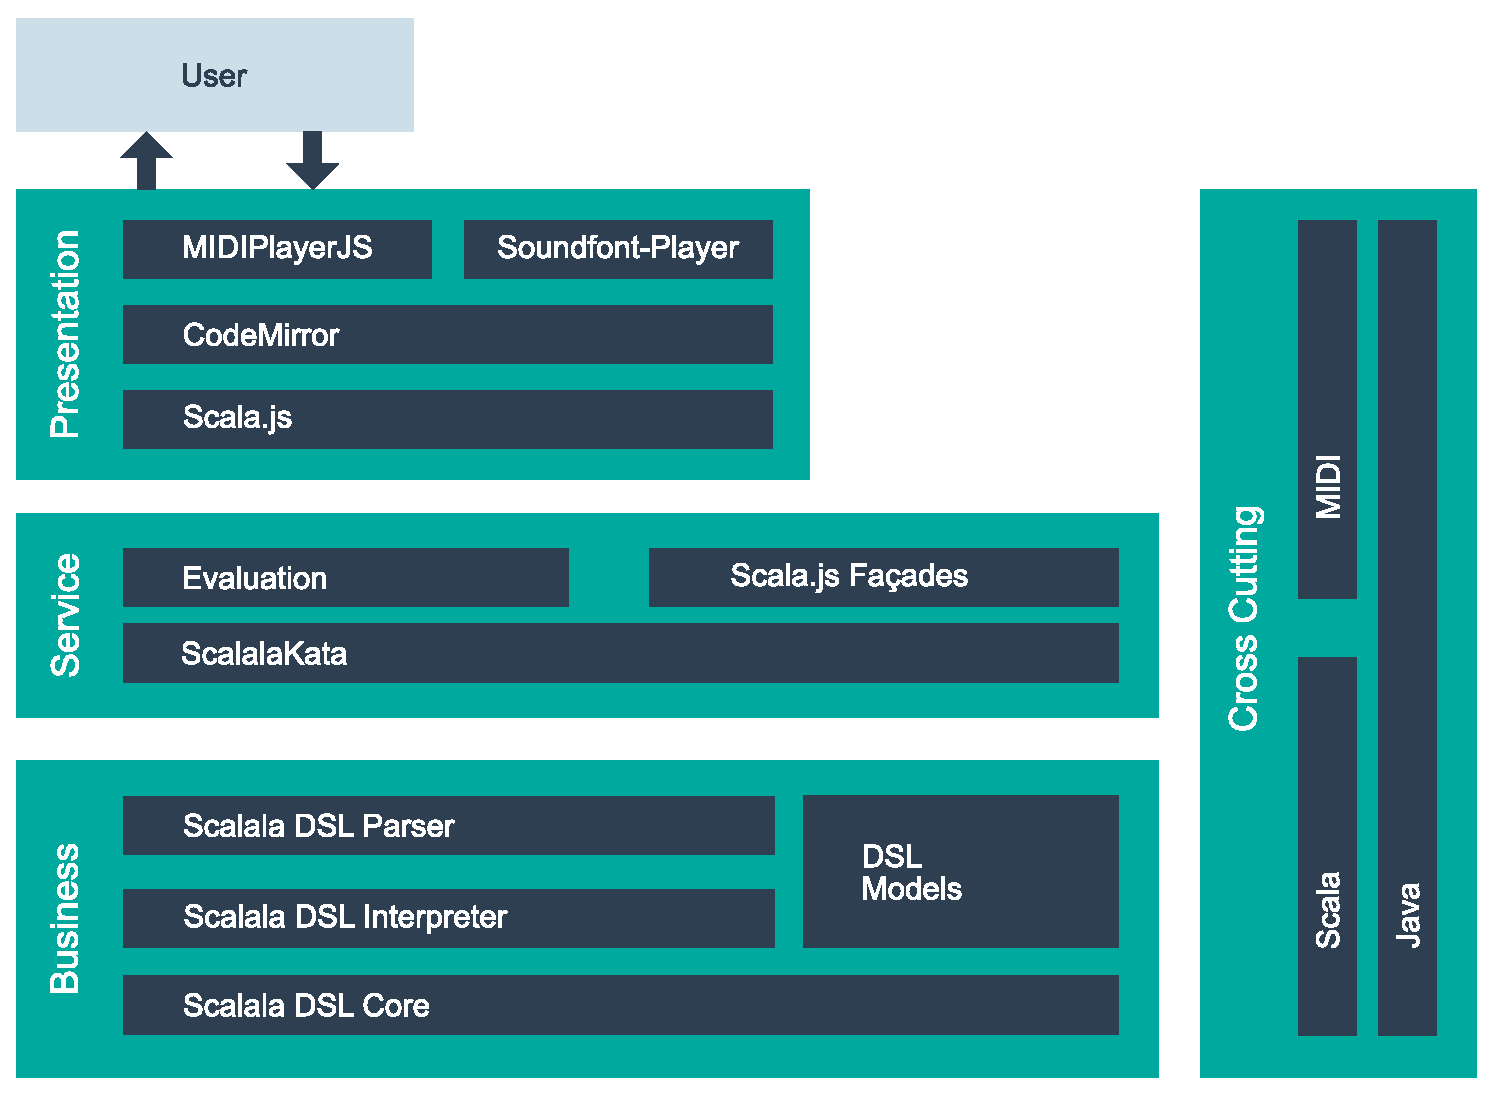
\includegraphics[scale=0.58]{app_layer}
\end{figure}

As seen in the diagram above, the application was implemented in a layered model. Contrary to modern architectures, this application does not follow the microservice-based approach, since the in this thesis implemented system consists of two parts:

\begin{itemize}
\item the web-application en bloc (Service and Presentation Layer) \newline Based on ScalaKata2 (cf. \ref{LIT_PROJ_SCALAKATA2})
\item the DSL library (Business Layer) \newline Based on Scalala (cf. \ref{LIT_PROJ_SCALALA})
\end{itemize}

The layered model was chosen to make use of the simplicity of this architecture and since it is a perfect fit for the classic client server relationship at hand. The DSL library itself was implemented in a model-controller approach (see next section).

The web-application was based on ScalaKata2. According to the advantages of Scala.js, the whole presentation layer was realised through Scala.js. To avoid mixing the Scala.js code base with native JavaScript code, Scala.js façades were written, which would otherwise necessary through the usage of third-party JavaScript libraries. The detailed implementation of the façades is explained in section \ref{IMPL_SCALALAKATA_CSMODEL_CLIENT}. The sound playback through the browser is represented through two libraries: MIDIPlayerJs\footnote{MIDIPlayerJs - \url{https://github.com/grimmdude/MidiPlayerJS}} and Soundfont-Player\footnote{Soundfont-Player - \url{https://github.com/danigb/soundfont-player}}.

Scala as GPL and the MIDI standard was used across all layers (cf. figure \ref{IMG_LAYER_ARCH}). Each layer was implemented in Scala, even the presentation-layer through Scala.js, and the MIDI standard was used to write audio on the DSL side and to read the audio sequences on the front-end side.

\section{DSL Library}
\label{ARCH_DSL}
This section briefly describes the DSL architecture. The DSL follows the \textit{Interpreter} approach. The DSL library reads the DSL script (the input) through the implemented \textit{Reader} at the \textit{Parsing Layer}, which translates the formal input into instructions for the GPL.\cite{Riti2018} The layer acts as the \textit{Lexical Parser} which creates the Abstract Syntax Tree (AST). The AST is used by the interpreter which walks through the AST and translates the results into MIDI. Beyond the theoretical modules, the DSL library, especially the translator relies on a decoupled MIDI class, which is used to create the MIDI result. The results of the MIDI layer could be a hard-disk file, the file encoded as Base64, or other. Besides the specific DSL Layer, each layer uses the already existing Models from Scalala (cf. \ref{THEO_SCALA}). Figure \ref{IMG_DSL_ARCH} illustrates the explained behaviour.

\begin{figure}[h]
\caption{Scalala DSL Architecture}
\label{IMG_DSL_ARCH}
\includegraphics[scale=0.7]{dsl_layer}
\end{figure}

\section{Sequence Model}
\label{ARCH_SEQ}
One outstanding feature of the applications architecture is the usage of the query result, especially the MIDI response. Since MIDI-streams are not possible to playback directly by the browser-engine, an approach to playback these files through JavaScript was necessary. To solve this circumstance, two libraries were included. The MIDIPlayerJs converts input sequences first to the JSON format and provides JavaScript events for each MIDI event. These JavaScript events are caught from the Soundfont-Player library to communicate with the browsers \texttt{AudioContext} and playbacks each MIDI event. Figure \ref{IMG_SEQ_ARCH} shows how a user interacts with the entire system.

\begin{figure}[h]
\caption{ScalalaKata Sequence Diagram}
\label{IMG_SEQ_ARCH}
\includegraphics[scale=0.47]{sequence_diagram}
\end{figure}





















\chapter{Implementation}
\label{IMPL}
The implementation is structured in two main parts:

\begin{itemize}
\item the DSL, called \textit{Scalala}
\item the Web-Application, called \textit{ScalalaKata}
\end{itemize}

The first section describes the overarching DSL implementation. It starts by explaining the concept of the language, discussing design aspects and the final implementation in Scala. The section then proceeds to introduce the web-application and each component of it. It explains the client-server implementation; particular attention is paid to the Scala.js sections. Both, the DSL and Web-Application, are merged in chapter \ref{RESULTS} to provide the holistic approach as a result of combining each component.

The interested reader is invited to read along in the project's source code at GitHub\footnote{ScalalaKata - \url{https://github.com/FunkeMT/ScalalaKata}}, to compare the illustrated concepts and verify the following chapters themselves.

\section{Scalala}
\label{IMPL_SCALALA}
The DSL was implemented through the Scala GPL. However, this study should not give an introduction to Scala programming; rather, provide the DSL realisation through Scala as host language. Therefore, only the DSL relevant Scala features are emphasised and explained. The design process of a DSL was carefully evaluated and adopted from Mernik's et al. research.\cite{Mernik2005} He described five phases of DSL development and identified patterns in each phase. His patterns are not a guideline on how to implement a DSL in detail, instead of guiding the decision process. The subsections of this section are named and organised by Mernik's pattern-based implementation:

\begin{itemize}
\item Decision
\item Analysis
\item Design
\item Implementation
\item Deployment
\end{itemize}

The name \textit{Scalala} is adopted from the related project Scalala. It is a neologism, which consists of the GPL name \textit{Scala} and the onomatopoeia \textbf{la}. This onomatopoeia alludes to the \textbf{la-la} syllables in songs.

\subsection{Decision}
\label{IMPL_SCALALA_DECISION}
The related projects in section \ref{LIT_PROJ} already emphasised that there is no available programming language or holistic approach according to the thesis requirements defined in \ref{INTRO_SOFT}. Furthermore, the aim of this study is to \textit{create a user-friendly notation} and to \textit{transform} notes, which are usually described through visual sheet notes. In conclusion, these aspects map identically with Mernik's "Notation Pattern" and supports the decision to create a new "domain notation".\cite{Mernik2005}

To fulfil the results of Soloway's\cite{Soloway1982}  and Kranch's\cite{Kranch2012} research and create a novice-friendly programming language close to the natural language, the cardinality of external DSLs was used. In addition, external DSLs are more powerful and more flexible by nature (cf. \ref{THEO_DSL}).

\subsection{Analysis}
\label{IMPL_SCALALA_ANALYSIS}
Comprehensive analysis is necessary to create a fundamental groundwork for the DSL implementation. The target domain, or "problem domain" has to be carefully examined. The problem domain contains all major artefacts like processes, entities and constraints, which are part of the target business. The process is necessary to create a "common language" between domain expert and developer, to provide communication and prevent errors.\cite{Ghosh2010}

According to this, the "common vocabulary"\cite{Ghosh2010} or "common dictionary"\cite{Riti2018} was developed. An extract of the developed vocabulary is illustrated in table \ref{TBL_COMMONDICT}. Also, the common vocabulary was used to model the "solution domain" which provides all tools, to solve the present problem.\cite{Ghosh2010, Riti2018}

Figure \ref{IMG_DSL_DOMAINS} illustrates the relationships between all named domains and shows, how the common dictionary is used in both domains and acts as the "glue" between both.\cite{Ghosh2010} Even though this comprehensive process is fundamental work, Mernik classifies this process as the most used "Informal Analysis Pattern", since extensive studies or surveys with the target domain were not performed by this project.\cite{Mernik2005}

\begin{table}[h]
\caption{DSL Common Dictionary (truncated). All "Translations" are simplified.}
\label{TBL_COMMONDICT}
\begin{tabular}{l|p{200pt}|l}
\rowcolor{htwg-teal} 
\textbf{Problem Domain}      & \textbf{Translation}		& \textbf{Target Domain}     \\
full score                  						& Sheet music, which contains all instruments and voices. Arranged in a fixed order. 		& track \\
instruments /  voices 					& A specific instrument which is played by a specific person.							& musician \\
octave 											& 	An interval between two pitches.																						& octave \\
note													& combination of pitch and duration.																						& note (a-g) \\
. . .													& . . . 																																			& . . .
\end{tabular}
\end{table}

\begin{figure}[h]
\caption{Common Dictionary as Glue beteween Problem and Solution Domain.\cite[p. 15]{Ghosh2010}}
\label{IMG_DSL_DOMAINS}
\includegraphics[scale=0.5]{dsl_domains}
\end{figure}



\subsection{Design}
\label{IMPL_SCALALA_DESIGN}
As mentioned in the section before, part of designing a language is to create the solution domain. In this thesis, the solution domain was created by defining the language concepts and the basic DSL architecture. Since the approach is to create an external DSL, according to the "Language Invention" pattern, the language has to be developed from scratch. The automatic generation through modern language generation systems was not possible, because of the "informal" notation and characteristics.\cite{Mernik2005} The language was suitably designed to satisfy both domains:

\begin{itemize}
\item Developer Domain \newline According to Riti's suggestions, the architecture was developed to encapsulate and hide implementation details to reveal only the parts which are necessary to solve the problem. Further, the system was designed to be easily maintainable.\cite{Riti2018}

\item Novice Domain \newline As suggested by Kranch, the language was designed close to the natural language. The reason to design the language as close to the natural language as possible was that Kranch's researches with novices illustrate, that his subjects applied their knowledge from natural languages to make an analogy to the program elements.\cite{Kranch2012} Another requirement to the language was to teach fundamental programming concepts; like variable declaration/usage, basic arithmetic and method invocation.
\end{itemize}

Because of the absence of any precise definition in the literature, in which stage the final language grammar should be developed, in the design or in the implementation phase, the chosen approach was to define the grammar during the design phase. However, the grammar has to be designed decoupled of the final implementation.  This can be attributed to the grammar definition language—Extended Backus-Naur Form (EBNF)—which exists independently from any implementation or language in general. Listing \ref{LS_EBNF_TRUNC} highlights the root rule and the sub-rules.

\begin{lstlisting}[caption={EBNF (truncated).}, label=LS_EBNF_TRUNC]
(*** Terminals ***)
INSTRUMENT		::=	'instrument';
MUSICIAN		::=	'musician';
TEMPO			::=	'tempo';
WITH			::=	'with';
TEMPO			::=	'tempo';

STRING	::=	[a-z]+;
INT	::=	[0-9]+;


(*** Non-Terminals ***)
identifier	::=	STRING;
song		::=	(musician)* track;   
track		::=	PLAY (tempo)? musicVars;
tempo		::=	WITH TEMPO INT;
musicVars	::=	musicVar (COMMA musicVar)*;
	
. . .
\end{lstlisting}

\subsection{Implementation}
\label{IMPL_SCALALA_IMPL}
Mernik's "Interpreter" pattern was chosen to implement the DSL since the aim is to develop an external one; thus, it is necessary to provide a "fetch-decode-execute cycle". This cycle describes, in general, the input fetching through the lexer, decoding this input through the parser and the final translation into code. Besides, the advantages are simplicity, greater control over the execution environment and maintainability. The disadvantages, like the considerable effort to implement a complex language processor or the risk to end in an incoherent design, were found to be acceptable.\cite{Mernik2005}

The implementation process can be summarised as followed (cf. \cite{Ghosh2010}):

\begin{figure}[h]
\centering
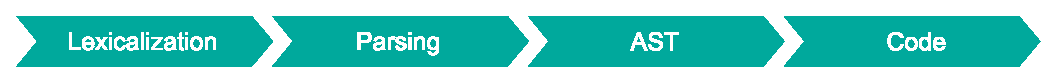
\includegraphics[scale=0.7]{impl_process_0}
\end{figure}

To be able to discuss each phase in more detail, the model is further divided into two layers:

\begin{itemize}
\item\textbf{1st Layer} Syntactic Analysis
\item\textbf{2nd Layer} Semantic Model
\end{itemize}

\subsubsection{Syntactic Analysis}
\label{IMPL_SCALALA_IMPL_SYNTACTIC}
The in EBNF notation modelled grammar was the starting point for the implementation. Based on this grammar, it is necessary to create the \textit{lexer}, also called \textit{tokeniser}, which handles the lexical analysis. The lexer splits an input stream into lexical units—the tokens. These tokens are the input of the parser. The parser generates a semantic model of the language and translates it into software.

The terms lexer and parser are often mixed and interchanged in the literature, since both have much in common. Moreover, a parser could act as the tokeniser for the next parser and so on. The main difference between both is the grammar:

\begin{itemize}
\item Lexer accepts regular grammars (Chomsky's level 3)
\item Parser accepts context-free grammars (Chomsky's level 2)\cite{Wagenknecht2014}
\end{itemize}

Due to the fact, that this study is not an introduction into language grammars, rather than in language design and implementation, the Chomsky hierarchy is not further explained. Wagenknecht et al. provides an overall introduction to language theory.\cite{Wagenknecht2014}

Depending on the complexity of the language, it could be a massive effort to create the lexer and the parser.\cite{Ghosh2010} This is one reason, why the DSL was developed through Scala; the Scala GPL offers the \textit{Parser Combinators} as a standard library which provides simple ways to create the abstraction model for the interpreter.

As an alternative to the parser combinators, it is possible to create the lexer \textbf{and} the parser through \textit{Parser Generators} like ANTLR\footnote{ANTLR - \url{http://www.antlr.org}}. The generators are tools with own configuration languages and settings.

\begin{figure}[h]
\centering
\includegraphics[scale=0.7]{impl_process_1}
\end{figure}

The lexer and parser were implemented in pure Scala, without any external tools or frameworks.\cite{Schmitt2014} Firstly the \textit{lexical parser} was developed to identify the lexing. The main idea behind the parser combinators is to define different parsers and \textit{combine} these to create one comprehensive parser.\cite{Riti2018} As mentioned before, lexing and parsing share many commonalities and are especially hard to isolate within the parser combinators; nevertheless, the lexer was implemented through extending the \texttt{StandardTokenParsers} class in according to Gosh and Riti.\cite{Ghosh2010, Riti2018} The lexer can be understood as the smallest parser unit. Through defining \textit{reserved} words and delimiters or using predefined parsers (like \texttt{numericLit} which defines numeric literal tokens), the lexer knows which chunk should be part of the input token stream. In the thesis's case, all reserved words were adopted from the EBNF terminal symbols. An extract of this lexer definition is illustrated in the listing \ref{LS_RESERVED_WORDS} below.

\begin{lstlisting}[caption={Defining the reserved words and delimiters through Scala's \texttt{StandardTokenParsers}}, label=LS_RESERVED_WORDS]
lexical.reserved += ("loop",
    "chord",
    "notes",
    "instrument",
    "musician",
    "with",
    "play",
    "plays",
    "tempo",
    "at",
    "c", "d", "e", "f", "g", "a", "h"
  lexical.delimiters += (",", "(", ")", "/", ".", "+", "-")
\end{lstlisting}

These predefined \textit{lexical parsers} are the groundwork for combining these parsers with other parsers.

\begin{figure}[h]
\centering
\includegraphics[scale=0.7]{impl_process_2}
\end{figure}

To apply the designed context-free grammar from \ref{IMPL_SCALALA_DESIGN}, Scala's parser combinators were utilised to define recursive descent (RD) parsers. RD parsers are the representation of \textit{recursive} functions to parse a tree starting at the top, ie. a top-down design (for further informations see Wagenknecht et al.\cite{Wagenknecht2014}). This parser is a direct implementation of a LL-parsers for LL(k)-grammars (usually $k = 1$).\cite{Ghosh2010}

The parser combinator offers the possibility to define a parser, which looks like an EBNF and its production rules. This is also the place where Scala proved to be very usefull since the parsers could be implemented with higher-order functions. This circumstance reduces redundant code considerably and provides the creation of small parser parts, each decoupled from another and composes them functionally to generate one large parser. Listing \ref{LS_PARSER_INIT} illustrates the first production rules which represent the initial parser rule (simplified). The names were adopted directly from the predefined EBNF; it is essential to apply this names, as suggested by Gosh because the rules reflect the domain concept and the "blueprint" to communicate with the domain experts.\cite{Ghosh2010}

\begin{lstlisting}[caption={Initial parser combinator rules. (simplified)}, label=LS_PARSER_INIT]
lazy val song		=	rep(musician) ~ track

lazy val musician	=	"musician" ~> ident

lazy val track		=	"play" ~> repsep(musician, ",")
\end{lstlisting}

The defined parser \texttt{song} already consists of two further parsers, \texttt{musician} and \texttt{track}, each of them represents a combination of further parsers, and so on. The elements are described as follows:

\begin{itemize}
\item\texttt{rep(musician)} \newline Repeats  \texttt{musician}   one or more times.
\item\texttt{repsep(musician, ",")} \newline Repeats  \texttt{musician}   one or more times with the separator  \texttt{","}.
\item\texttt{"musician"} \newline Represents a  \texttt{keyword}   which was defined at the  \texttt{lexicalization}   (cf. Lexicalization) and is parsed through the  \texttt{lexer parser}.
\item\texttt{"play"} \newline Same as  \texttt{"musician" }.
\item\texttt{ident} \newline Also a lexer representation which matches an identifier (String).
\end{itemize}

Each parser, like \texttt{rep(musician)} or \texttt{track}, composes a DSL syntax parser sequentially. To combine each of them, \textit{combinators} are applied (represented as higher order functions). Combinators are represented through symbols for brevity and implemented as methods within the Scala class \texttt{Parsers[T]}.\cite{Ghosh2010}

Presumed \texttt{P} and \texttt{Q} are parsers, they can be combined as shown in table \ref{TBL_COMBINATORS}. Note, however, that this table represents only the common productions rules, and is not complete.

\begin{table}[h]
\caption{Scala Parsers (truncated).\cite{Riti2018}}
\label{TBL_COMBINATORS}
\begin{tabular}{l|l|p{180pt}}
\rowcolor{htwg-teal} 
\textbf{Parser}      & \textbf{Name}		& \textbf{Description}     \\
\lstinline|P ~ Q|						& Sequence 					& \texttt{P} consumes the first part of the input stream, followed by \texttt{Q}, which consumes the remaining part from \texttt{P}. \\
\lstinline|P ~> Q|		 					& Selective Sequence	& Works like \lstinline|~|, but returns only the result from \texttt{} Q. However, \texttt{P}'s presence is necessary but can be dropped from the result. \\
\texttt{P | Q}								& Alternation					& Acts identically to the EBNF \texttt{|} symbol which represents an \texttt{OR} connection between two parsers.
\end{tabular}
\end{table}

To transform an input into a result, each parser implements the methods \texttt{Success}, \texttt{Failure} and \texttt{Error}. This allows the parser to use \textit{backtracking}. For example, the parser combinator \lstinline|P ~ Q| can be explained as follows (cf. \cite{Ghosh2010}):

\begin{itemize}
\item If \texttt{P} ends in \texttt{Success} then, and only then, \texttt{Q} is examined and is fed with the truncated input stream.

\item If \texttt{P} ends in \texttt{Failure}, the input stream can not be matched with this parser, \texttt{Q} is not further examined and, backtracking is invoked to try alternative rules—if there are any available.

\item If \texttt{Failure} is fatal or another runtime exception happens, \texttt{Failure} ends in \texttt{Error}, no backtracking is done, and the process returns.
\end{itemize}

This short example, as well as table \ref{TBL_COMBINATORS} and listing \ref{LS_PARSER_INIT}, however, disclose already the disadvantage \textbf{and} advantage of Scala's parser combinator: the short syntax and its accompanying readability.

The combinator symbols utilize another Scala feature, called infix operation notation, and are predefined methods within the class \texttt{Parsers[T]}. If the infix notation is suppressed, the sequence combinator \lstinline|P ~ Q| would be a simple method call \lstinline|P.~(Q)|. This notation allows exact and short code and to model the parser similar to the EBNF notation.\cite{Ghosh2010}

The parser represents the DSL's core junction between the designed language through EBNF notation and the programming language. To create the AST, the current layer \textit{Syntactic Analyse} is left, and the further steps are explained in the following layer—\textit{Semantic Model}.

\subsubsection{Semantic Model}
\label{IMPL_SCALALA_IMPL_SEMANTIC}

\begin{figure}[h]
\centering
\includegraphics[scale=0.7]{impl_process_3}
\end{figure}

The essential part to create the connection between the parsed structure, the grammar and the final output, is to generate the semantic model in memory which is the actual result of the parser. The semantic model is usually an AST. Each node in the tree represents a token which is used in the grammar. Using the method of Riti, a homogenous AST was implemented, since it is the most straightforward approach to walk through the AST and generate the final code.\cite{Riti2018}

To create this tree, the implemented parser was extended to transform the result of a particular parser in such way that the semantic model is built incrementally. Through \textit{function application combinators} the parser applies functions to the parsed input stream. Listing \ref{LS_PARSER_FUNC} illustrates the extended version of listing \ref{LS_PARSER_INIT} with \textit{function application}.

\begin{lstlisting}[caption={Parser combinator rules extended through \textit{function application}.}, label=LS_PARSER_FUNC]
lazy val song: Parser[Song] = rep(musician) ~ track ^^ {
	case m ~ t => Song(m, t)
}

lazy val musician: Parser[Musician] = "musician" ~> ident ^^ {
	case m => Musician(m)
}

lazy val track: Parser[Track] = "play" ~> repsep(musician, ",") ^^ {
	case m => Track(m)
}
\end{lstlisting}

Again, the symbol \lstinline|^^| is just a method call, shortened through infix notation.\cite{Ghosh2010} The return value of an applied function matches the defined return value from the parsers signature (implicit). Scala's \textit{case classes} functionality directly supports the AST creation by matching the succeeded parser and assigning the matched values to an object. However, to create the AST representation as described, the underlying semantic model has to be predefined. Simplified, the semantic model is just plain Scala and represents all traits, case classes and objects which are in use. Finally, the AST is the result from the parser itself and allows the translator to \textit{walk} through all objects and create the output.


\begin{figure}[h]
\centering
\includegraphics[scale=0.7]{impl_process_4}
\end{figure}

The final output generation is the last step in converting an input DSL script into code and is handled by the interpreter. In the thesis's case, the output is the MIDI sound file. To convert the AST in actual output, the \textit{tree-pattern-matcher} was used.\cite{Riti2018} The AST is walked through recursively, and through pattern matching, an action is invoked at the relevant term. The graphical representation of this \textit{process} is the translation result of the input DSL script example in listing \ref{LS_DSL_WALK} and is illustrated in figure \ref{IMG_DSL_AST}. The MIDI generation is explained in section \ref{IMPL_SCALALA_MIDI}.

\begin{lstlisting}[caption={DSL script example.}, label=LS_DSL_WALK]
musician pianist_1
   instrument Piano
   plays c,d,e

play with tempo 60
   pianist_1
\end{lstlisting}

\begin{figure}[h]
\caption{DSL script example - AST.}
\label{IMG_DSL_AST}
\includegraphics[scale=0.57]{ast}
\end{figure}





\subsection{Deployment}
\label{IMPL_SCALALA_DEPL}
In this study, the DSL was deployed as a Scala library. Thus, an easy to apply deployment mechanism to continuous integration tools like \textit{Travis-CI} is possible and the integration into other applications is straightforward.
\newline
\newline
This section illustrated, how the DSL was designed from scratch and implemented by the Scala parser combinator. To conclude, Mernik's decisions guideline\cite{Mernik2005} through patterns provided an excellent basic structure in DSL development. The Scala parser combinators are a reliable approach to implement an external DSL. Through functional programming and pattern matching, an abstraction of the defined grammar was easy to implement. However, since there is no official comprehensive documentation for Scala's parser combinator, it was very time-consuming to become familiar with the library and achieve results.


\subsection{MIDI}
\label{IMPL_SCALALA_MIDI}
In addition to the \textit{code generation} part of the DSL implementation, the interpreter was also implemented as the generator of the sound result. As already mentioned before, the DSL was implemented on top of the related project Scalala, which already provides the necessary MIDI representation. For the sake of simplicity, some parts of the semantic model rely on the Scalala model and were reused. Since Scalala represents an internal DSL, the implemented external DSL was developed on top of the internal one, which is a frequently used approach in the literature (cf. \cite{Fowler2010}).

While the interpreter is \textit{walking} through the AST recursively, the MIDI representation is constructed incrementally. The MIDI generation process was implemented as a plain Scala class which builds up the basic MIDI file structure and provides public methods to add notes, switch the instrument, set the tempo, etc. The implementation was done according to the MIDI-standard description.\cite{MIDIManufacturersAssociation} As in \ref{THEO_MIDI} described, the MIDI-protocol is constructed through byte-data sets and messages. This approach offers a fully flexible way to create MIDI-sound-files. However, the implementation, as well as the debugging at the byte-level, is less than ideal. Since the MIDI-file represents a binary file, it is not possible to comprehend which sequences were written to the file; a third-party application is necessary to decode the file, examine its contents and verify the correctness. In the thesis's case, the MacOS application \textit{MidiMusicXmlPlayer}\footnote{MidiMusicXmlPlayer v1.60 - \url{http://programfabriken.com}} was used and provided excellent results in MIDI decoding and playback.














\section{ScalalaKata}
\label{IMPL_SCALALAKATA}
The web-application ScalalaKata provides a user interface to write a DSL script textually and invoke its interpretation. As already mentioned, the application is based on ScalaKata2, since it is a well-suited foundation for this thesis. First, the underlying technologies are briefly explained. The chapter then proceeds to illustrate the client-server-model. Particular attention is paid to the client, since Scala.js as front-end technique was used. The last paragraph elaborates on the deployment of the application.

The name \textit{ScalalaKata} was inspired by the related project \textit{ScalaKata2}. It is a compound of the used DSL \textit{Scalala} and the Japanese word \textit{Kata}. Literally, Kata means \textit{form} and refers back to martial arts and exercises consisting of sequences which are repeatedly practised. Thomas adopted this term to Code Kata to learn and train programming by repeating code snippets over and over.\cite{Thomas2013}

\subsection{Technologies}
\label{IMPL_SCALALAKATA_TECHS}
ScalalaKata also uses Scala as GPL; thus a seamless DSL integration and the creation of a consistent ecosystem is provided. Through the \textit{Akka}\footnote{Akka - \url{https://akka.io}} toolkit, Scala offers a full server- and client-side HTTP stack. ScalaKata2 is already pre-configured and implements a primary Akka HTTP server in combination with Scala.js as client.

The front-end is styled through \textit{Less}\footnote{Less - \url{http://lesscss.org}}. Less is a language extension for CSS. Less consists of the Less language and the Less.js JavaScript tool to convert the Less syntax into valid CSS styles.\cite{Lesscss.org}

To provide an incremental compilation, a local as well as published dependency management and deployment mechanism, the \textit{sbt}\footnote{sbt - \url{https://www.scala-sbt.org}} build tool was chosen. Sbt is the standard build tool for Scala and Java projects. Through the incremental compilation, sbt provides a gentle performance and performant recompilation, since it compiles only affected files and dependencies.\cite{LIGHTBENDINC} Sbt, in combination with \textit{node.js}\footnote{node.js - \url{https://nodejs.org/en/}}, accomplishes the converting process for Less and compilation of Scala.js code.

\textit{CodeMirror}\footnote{CodeMirror - \url{https://codemirror.net}} represents the main front-end component. It enables the writing of the DSL script in a web environment. CodeMirror is an adjustable text editor, written in JavaScript, for editing code in the browser.\cite{Codemirror} CodeMirror offers syntax highlighting for the most common programming languages and the opportunity to define new highlighting through RegEx definitions. Furthermore, in-code annotations are available to place error messages or code evaluations in-line.

To playback sound through MIDI in web-environments, third-party JavaScript libraries are necessary. As already mentioned in \ref{ARCH_SEQ}, MIDIPlayerJs converts a MIDI binary file into a higher abstraction. The Soundfont-Player library uses this abstraction in combination with pre-defined soundfont-files to playback sound.

\subsection{Client-Server Model}
\label{IMPL_SCALALAKATA_CSMODEL}
The entire ScalalaKata application follows the standard model for web-applications. In particular, the application was divided into server and client part.

\subsubsection{Server}
\label{IMPL_SCALALAKATA_CSMODEL_SERVER}
The server part is almost negligible since it represents a simple server solution through Akka HTTP to receive HTTP requests, process the request and answer with a response; regardless if the request ends in an error or not. This process can be verified again by consulting the sequence model from \ref{ARCH_SEQ}. All messages were packed into the JSON notation to provide a generic approach; request, process and response can be explained as follows:

\begin{itemize}
\item\texttt{Request}\newline
The request consists of a simple string representation of the written DSL script inside the CodeMirror browser instance.

\item\texttt{Process}\newline
The request is directly forwarded to the Scalala DSL, without previous modifications. The DSL returns the Scala parser combinator with the result as \texttt{Success}, \texttt{Failure} or \texttt{Error}.

\item\texttt{Response}\newline
Based on the Scalala DSL result, the response is packaged differently. \texttt{Success} passes the generated MIDI file and adds it to the response—base64 encoded. \texttt{Failure} and \texttt{Error} create a response with the exception message and tries to add the position where the exception happened. Thus, the exception message can be later displayed at the exact code position in the CodeMirror browser instance.
\end{itemize}

\subsubsection{Client}
\label{IMPL_SCALALAKATA_CSMODEL_CLIENT}
The client implementation was very time-consuming since there is no standard approach to playback MIDI in web-environments. The interaction of both JavaScript libraries, MIDIPlayerJS and Soundfont-Player, provides a good solution to work around this problem.

The MIDIPlayerJS library creates an intermediate layer between the MIDI binary file and the browser engine's \texttt{AudioContext} in JSON. For each control sequence within the MIDI file, the library adds an appropriate node representation to the JSON. This builds the JSON structure incrementally. MIDIPlayerJS holds an own time representation, and the events are fired at the right time according to the generated MIDI sequence.

The Soundfont-Player communicates directly with the browser engine \texttt{AudioContext}, which is a complex oscillator by its own and able to control the hardware of the underlying device to generate sound. Through external soundfonts, the library can play sound at a specific \texttt{AudioContext} time. Soundfonts are simple music files, like mp3 and contain, for a specific instrument, all relevant sound representations. This also implies that the sound quality depends on the loaded soundfont. The Soundfont-Player subscribes to events which are fired by the MIDIPlayerJS.

To combine all explained libraries and develop a comprehensive application, native JavaScript code is necessary on the client-side. Due to the underlying Scala environment, Scala.js was used to write the client in a type safe and error reporting manner. To prevent having to write native JavaScript in the client logic, Scala.js façades were utilised. Façades types are similar to TypeScript type definitions. Through native Scala traits and classes, the JavaScript API is mapped with zero overhead to the Scala language—but in a type-safe way.\cite{ScJsDoc}

For the most popular libraries or the used CodeMirror, façade types were already implemented by the open-source community and available as simple sbt library dependencies. For less popular libraries, like the MIDIPlayerJS and Soundfont-Player, an own implementation was unavoidable. To state one advantage: It is not necessary to implement the entire JavaScript library API as a façade, only the used and needed API parts have to be implemented. The implementation is based on annotations and the naming of the traits and methods in the global context. During compile time, the Scala.js compiler tries to map the written façade type to the linked libraries. Through that, it was possible to write Scala.js and use type-safe façade classes within the client logic. Figure \ref{LS_JS_SCALAJS_FACADE} and \ref{LS_SCALAJS_FACADE} compares the native JavaScript API to Scala.js façades.

\begin{lstlisting}[caption={MIDIPlayerJs \texttt{Player} API as native JavaScript}, label=LS_JS_SCALAJS_FACADE]
new Player(eventHandler, buffer)

loadFile(path)
loadDataUri(dataUri)
play()
stop()
setTempo(tempo)
getSongPercentRemaining()
\end{lstlisting}

\begin{lstlisting}[caption={Scala.js Façade for the MIDIPlayerJs class \texttt{Player}}, label=LS_SCALAJS_FACADE]
@js.native
@JSName("MidiPlayer.Player")
class Player(eventHandler: js.Function = null, buffer: js.Array[Any] = null) extends js.Object {

  def loadFile(path: String): Player = js.native
  def loadDataUri(dataUri: String): Player = js.native
  def play(): Player = js.native
  def stop(): Player = js.native
  def setTempo(tempo: Int): Unit = js.native
  def getSongPercentRemaining(): Int = js.native

  def on(eventName: String, handler: js.Function): Unit = js.native
}
\end{lstlisting}


\subsection{Deployment}
\label{IMPL_SCALALAKATA_DEPLOY}
Each developed library, MIDIPlayerJs-Façade, Soundfont-Player-Façade and the Scalala DSL were deployed to public repositories through uploading the corresponding artefacts to a software distribution service\footnote{JFrog Bintray Software Distribution Service - \url{https://bintray.com}}. The main advantage of this solution is that the ScalalaKata application can be cloned and built, without other necessary local dependencies. Furthermore, the developed façades are now part of the Scala.js pre-defined façades and available for the open-source community.

The Scalala DSL is further connected to \textit{Travis-CI}\footnote{Travis-CI - \url{https://travis-ci.org}}, a continuous integration platform which provides information about the compilation status and test execution. Since the DSL is the central part of the holistic application, this connection provides a solution to keep the library on a safe build-status.

\textit{Docker}\footnote{Docker - \url{https://www.docker.com}} has proven to be the simplest way to deploy the ScalalaKata application, due to the number of sub-modules and dependencies like Scala.js and other. The Docker build process was essentially adapted to the build process in ScalaKata2 and was implemented through the sbt-plugin \textit{sbt-docker}. The plugin enables the build of a Docker image through the sbt build process. No further Docker configuration files are necessary. Besides, the plugin offers the possibility to provide the Docker image locally or publicly. The published libraries and façades support the Docker build process; they do not have to be available at the production web-server and are loaded directly from the distribution service.


























\chapter{Results}
\label{RESULTS}
In related studies, attempts were made to bring programming and teaching together through writing sound (cf. Sonic Pi \cite{Aaron2016Art}) or writing music (cf. Scalala). But all projects lack language fluency and assessibility. The primary purpose of this work was to create a domain-specific language to write music notation in an intuitive environment. The language was designed for novices in programming and novices in music. It is known from the literature that novices are seeking fluency to link programming constructs with natural language.\cite{Bonar1985}

To create such an environment, this thesis utilised the Scala parser combinators to define, implement and provide an external DSL library—Scalala—which converts an input DSL script into MIDI sequences. To provide an interactive user environment, a web-application, based on Scala Akka as server and Scala.js as client, was implemented. The application was forked from ScalaKata2, modified and released as ScalalaKata. As already outlined in chapter \ref{INTRO} only the combination of both yield the desired holistic application.

To reach this particular requirement, the DSL was developed as a stand-alone library and finally included as a dependency to the web application. Sbt dependency's and deployment management was used to publish Scalala and integrate it into ScalalaKata.

In this section, the results are presented in three main parts:

\begin{itemize}
\item Examining the designed language and reviewing fluency as well as usability.
\item Discussing the implemented web-approach and examining its accessibility.
\item Introducing a minor case study and discussing the results.
\end{itemize}

\section{Exploration of the DSL}
\label{RESULTS_DSL}
All following DSL script listings are illustrations from the final user interface ScalalaKata. As an overall result, figure \ref{IMG_SCREEN_M} presents an DSL script example.

The result demonstrates the definition and usage of one simple \texttt{musician} variable which holds an \texttt{instrument} and simple \texttt{notes}. Analysing the language regarding its fluency, the language strongly matches the analogy to plain English and meets the observations from Soloway.\cite{Soloway1982} If one statement is \textit{spoken} as a whole sentence, the correlation to plain English is already recognisable.

One of the aims of this thesis was to teach the fundamental programming concepts. The scope of the designed language and the provided programming principles are listed in table \ref{TBL_DSL_TEACHING}.

\begin{table}[h]
\caption{DSL notation and programming concepts.}
\label{TBL_DSL_TEACHING}
\begin{tabular}{p{200pt}|p{180pt}}
\rowcolor{htwg-teal} 
\textbf{DSL Notation}                  			& \textbf{Programming Concept}     \\
\texttt{note.[flat | sharp | dot]}            & Method invocation \\
\texttt{musician [var]}                   		& Variable declaration and usage \\
\texttt{[++ | - -]note}                    			& Prefix notation \\
\texttt{note / [2 | 4 | 8 | 16]}                 & Arithmetic \\
\texttt{musician [var1]}\newline\texttt{musician [varN]}\newline\texttt{play [var1] [varN]}		& Sequential programming \\
\texttt{chord([notes])}\newline\texttt{loop([notes])}  							& Arguments
\end{tabular}
\end{table}

Table \ref{TBL_DSL_TEACHING} also demonstrates the language cardinality related to the music cardinality. A music-domain expert should note, however, that the music notation range is not fully exploited and offers less notations than, for example, LilyPond (cf. \ref{LIT_PROJ_LILY}). Nevertheless, comprehensive music notation was not within the scope of this study, since the aim was to reduce complexity. Furthermore, the music notation represents only the metaphorical abstraction to conventional programming paradigms. For example, in table \ref{TBL_DSL_TEACHING}, \texttt{musician} is just a metaphor for the data type and variable definition in conventional programming. The metaphor approach is similar to Kahn's ToomTalkTM.\cite{Kahn1995}

Figures \ref{IMG_SCREEN_S}, \ref{IMG_SCREEN_M} and \ref{IMG_SCREEN_L} gives further examples in three complexity gradients—simple, intermediate and advanced.

\begin{figure}[h]
\caption{ScalalaKata Example \textbf{\romannumeral 1} - simple ("Twinkle, Twinkle, Little Star" - Jane Taylor)}
\label{IMG_SCREEN_S}
\includegraphics[scale=0.5]{screen_simple}
\end{figure}

\begin{figure}[h]
\caption{ScalalaKata Example \textbf{\romannumeral 2} - intermediate ("The Imperial March"- John Williams)}
\label{IMG_SCREEN_M}
\includegraphics[scale=0.5]{screen_intermediate}
\end{figure}

\begin{figure}[h]
\caption{ScalalaKata Example \textbf{\romannumeral 3} - advanced ("Believer" - Imagine Dragons)}
\label{IMG_SCREEN_L}
\includegraphics[scale=0.5]{screen_advanced}
\end{figure}

\paragraph{Simple}
Example \textbf{\romannumeral 1}  illustrates a DSL script in its simplest form. One \texttt{musician} and basic \texttt{notes} are used. This example already uses the concepts of variable definition and usage, lists and sequence programming. Advantages are the simplicity for both domains—programming and music novices. Disadvantages are the reduced capabilities in music composition.

\paragraph{Intermediate}
Example \textbf{\romannumeral 2} represents an intermediate implementation. In addition to example\textbf{ \romannumeral 1 }, optional parameter and method invocations were added. Advantages are higher flexibility in music and teaching of further programming concepts.

\paragraph{Advanced}
The advanced implementation, example \textbf{\romannumeral 3}, represents the entire spectrum of the language. Almost all constructs were used. As can be seen, the advanced syntax is less than perfect and may introduce some difficulties for novice programmers This complexity is in direct correlation with the music complexity.

\section{Web-Application}
\label{RESULTS_WEBAPP}
The web-application was implemented as in a cross-platform and responsive application with seamless DSL integration and Docker deployment. The usage of CodeMirror as main client library resulted in an optimal approach since CodeMirror is by default optimised for responsive applications and mobile environments.

Minor adjustments were made to provide MIDI support in cross-platform environments. By default, mobile browsers prevent playing audio through JavaScript. The user has to accept the playback and invoke the playback through an explicit interface interaction like touch gesture or click event. Because of this circumstance, in some browsers, the user has to execute the DSL script in its first instance by pressing the \texttt{play} button. After that the short-cut \texttt{Cmd + Enter} is available. Furthermore, the used \texttt{AudioContext} is not consistent across all browsers. Safari, for example, needs a different instantiation as the other engines\footnote{As of the date of publication of this thesis.}.

The web-appplication was implemented, according to the aim of this study, as an interactive solution. Compared to Sonic Pi (cf. \ref{LIT_PROJ_SONICPI}), ScalalaKata is not as interactive. In particular, Sonic Pi's advantage is a highly complex timing model, which pastes new code fragments during runtime at an calculated position, to provide a seamless transition.\cite{Aaron2014} Refer to chapter \ref{DISCUSSION} for a comprehensive discussion related to this issue.


\section{Minor Case Study}
\label{RESULTS_STUDY}
A minor case study was conducted. It should be noted, however, that this examination does not represent a complete and comprehensive case study since this is beyond the scope of this thesis. For further projects, a comprehensive study is recommended. Nevertheless, the examination revealed useful insights.

The ScalalaKata application was given to three independent users; each of them affiliated with a different domain.

\begin{itemize}
\item User A belongs to the programming domain only.
\item User B belongs to the music domain only.
\item User C belongs to the programming \textbf{and} music domain.
\end{itemize}

The users conducted the study under the same conditions:

\begin{itemize}
\item A brief introduction into the application's background was given.
\item There was no explanation in advance about syntax and usage.
\item An example DSL script was shown as an initial start script.
\item There was no defined goal. They were welcome to experiment freely.
\end{itemize}

A comprehensive table of the observed user behaviours and the report is given in appendix \ref{APPENDIX_A} and appendix \ref{APPENDIX_B}. To emphasise significant results, the following résumé relates some of the found insights to the literature.
\newline
\newline
In line with Kranch's observations, subjects from the programming domain analysed the program structure. The novice just concentrated on particular instructions and tried to derive rules from natural language to create a structure.\cite{Kranch2012} Furthermore, the programming novice named some instructions, like the \texttt{f.sharp}, by using language from the music-domain. The programming expert instead named these constructs using their programming knowledge: "I call a method of the note f". This observation is similar to Kranch's research. Kranch further mentioned that the novices "took up to three times as long as experts to analyse the short program in the study".\cite[p. 309]{Kranch2012} This observation was not met in this study: All three subjects took the same time to get familiar with the new syntax. One possible cause for this may be that the DSL language was also entirely new for the experts and they had to compare the syntax to their programming knowledge.

Beyond this, all subjects requested further guidelines regarding the syntax, since the example did not include a comprehensive syntax overview, and all subjects wanted to implement more complex music constructs. Thus, it can be concluded that the initial example script is not sufficient as a guideline. A comprehensive guidebook or more examples may be necessary.

Another interesting observation was that the programming and music expert mentioned that he/she did not compare the language to a programming language, and he/she thought just in music notation. Thus, the subject intuitively wrote  \texttt{cis} instead of thinking about method invocation. This observation supports the fluency of the DSL language and the proximity to the natural language.

Besides, all subjects stated that the error messages were not useful. In future, comprehensive exception handling and user-friendly error messages should be implemented. Chapter \ref{DISCUSSION} gives an example to improve error message handling through the Scala parser combinators.

All users had no issues with the user-interface at all. Writing the script through the provided CodeMirror instance as well as the interaction through buttons (execute/play; stop), was no problem.

\section{Performance Analysis}
\label{RESULTS_PERFOMANCE}
This paragraph concludes the result chapter with a brief performance analysis. Especially the performance of the web-application is examined since there were significant performance anomalies. Due to the small language scope and the less amount of parsers, the external DSL Scalala is negligible for the analysis.

During implementation, the web-application was mainly developed and tested with the Google Chrome browser. After completing the first prototype of the ScalalaKata application, Mozilla's Firefox browser was also tested and significant performance issues in the music playback were recognised. Further examinations revealed that the MIDI playback is extremely resource intensive. The Firefox browser is not able to playback MIDI scripts accurately if more instruments are involved and the tempo is increased over 150 bpm. The CPU load of the Google Chrome browser and Mozilla's Firefox are compared in figure \ref{IMG_CPU_BROWSER}. As can be seen for Firefox, one CPU core is continuously at 100\% load, since the CPU scheduler switches the process from core to core. However, Firefox is based on the same \texttt{AudioContext} as the Google Chrome browser; it has not been possible to provide a definite answer to this circumstance. Nevertheless, basic MIDI scripts are possible, and all other state-of-the-art browsers, including mobile-browsers, are working without any performance issues.

\begin{figure}[h]
\caption{CPU load during the ScalalaKata app running and sound playing. (Test Setup: 4 Core CPU)}
\label{IMG_CPU_BROWSER}

\includegraphics[scale=2]{cpu_browser}
\end{figure}
















\chapter{Discussion}
\label{DISCUSSION}
The following chapter discusses the gained results and relates them to other research. Furthermore, this section should give some direction towards future work and discuss some limitations of the developed software.

In section \ref{IMPL_SCALALA} the implemented external DSL was explained in detail, and several example scripts were given and discussed. The decision to implement an external DSL was made since external DSLs offer a wide range of flexibility in the language grammar and there are no restrictions in defining a language close to the target domain vocabulary. Through the Scala parser combinators, a developed EBNF can be directly implemented, even though the familiarisation with this API took longer as excepted because of Scala's Parser Combinator's complex syntax. However, the resulting external DSL provides fluency and is comparable to plain English. Which is one key result from Kranch's\cite{Kranch2012} and Soloway's\cite{Soloway1982, Bonar1985} research in teaching novices programming. In chapter \ref{RESULTS_DSL} programming concepts were shown which can be taught to novices through this developed language.

The designed language fulfils the requirements in fluency and proximity to natural language. However, the cardinality of the music notation could be improved. Chapter \ref{INTRO} already mentioned that the defined DSL might not be a Turing complete language. Obviously, the final language is not Turing complete, since it is impossible to define simple functions or simple arithmetic expressions like $1 + 1$. However, the aim of this study was not to design a Turing complete language but a language which is less complex and may have not the ability of a full programming language or represents the full music bandwidth. An interesting question for further studies could be to examine and to question the correlation between Turing completeness and complexity in languages for novices.

Chapter \ref{RESULTS_WEBAPP} already illustrated, that ScalalaKata is not as interactive as Sonic Pi, because of Sonic Pi's timing model. The main disadvantage of ScalalaKata is that after one DSL script evaluation, the playback repeats from the top. Although this behaviour is evident and does not lead to a confusion of the user, it reduces interactivity. Further studies should examine if it is necessary and helpful to populate modifications interactively. One possible approach to reflect the changes would be to exploit the MIDIPlayerJs library, since this library is the first involved layer which converts the MIDI binary file into readable JSON. Whenever a new DSL script is evaluated, the new JSON could be compared to the last JSON and determine the modifications since the last evaluation.

In the minor case study, the error messages were criticised the most (cf. \ref{RESULTS_STUDY}). Future work should implement a comprehensive exception handling. The Scala Parser Combinators offer a simple way to provide custom error messages for each parser. As explained in \ref{IMPL_SCALALA_IMPL}, the \textit{function application combinators} are a powerful tool to create the semantic model. Besides, the \textit{combinator for \textbf{partial} function application} offers the opportunity to throw custom exceptions if a parser ends in an \texttt{Error} instead of \texttt{Success}. This enables the definition of custom messages for each parser.

Through ScalaKata2 as groundwork application and the extension through MIDI, ScalalaKata represents a comprehensive and convincing approach which is both intuitive and accessible. The application supports cross-platform and mobile devices. Contrary to Sonic Pi and LilyPond, there is no further installation or download necessary. Through the opportunity to access the system everywhere and at any time through mobile devices, the access for everyone was enabled.












\chapter{Conclusion}
\label{CONCLUSION}
A general introduction to this thesis, the topic and the research objectives were given in chapter \ref{INTRO}. To provide the reader with the underlying theoretical principles, chapter \ref{THEO} discussed the difference between internal and external DSLs and defined Scala as backbone GPL. Related literature was reviewed in chapter \ref{LIT} to provide a necessary background of the thesis's research field and to point out a gap in the current research. Besides, the chapter presented some related work and discussed their advantages as well as disadvantages in correlation to this thesis. Chapter \ref{ARCH} defined and explained the applications architecture. The defined requirements in \ref{INTRO_SOFT} were implemented in detail in chapter \ref{IMPL}. The results were extensively discussed in chapter \ref{RESULTS}, and a minor case study was given which provided useful results related to the DSL's properties. The discussion in chapter \ref{DISCUSSION} compared the developed DSL to Turing completeness, stated the advantages of the ScalalaKata web-application and raised questions for future work.

The thesis successfully implemented a holistic web-application, integrating the developed language Scalala. Therefore, the initial aim of this thesis was successfully achieved. An external DSL was developed for novices which can be used in an educational context. Fluency and proximity to plain English were achieved through consulting related studies and research in the field of teaching novices and children.

The web-application presents a cross-platform as well as a mobile approach to provide an accessible application for everyone. Through publishing the developed libraries to a software distribution service, this thesis has made a contribution to the open source community and enables further research.

The minor case study showed that the language is accessible to both domains and illustrated correlations to significant case studies from other research and stated the importance of comprehensive studies. The interviews with the music domain experts showed, that the developed language does not reach the full cardinality of the music domain and some language implementations do not fulfil all music domain requirements. This observation outlined the importance of the communication process between developers and domain experts in implementing a new language, which is stated by Fowler.\cite{Fowler2010}

Wing declared "Computational Thinking" a vital skill for novices and children.\cite{Wing2006} This could be applied to Schnabel's statement to provide the next-generation with fundamental knowledge.\cite{Schnabel2011} However, this thesis showed that the effort to create a new language from scratch and provide an accessible interface should not be neglected. Nevertheless, to create solutions which enhance "Computational Thinking" is worth the effort.




%% Use letters for the chapter numbers of the appendices.
\appendix

\chapter{Appendix - Minor Case Study Report}
\label{APPENDIX_A}

\begin{itemize}
\item User A belongs only to the programming domain.
\item User B belongs only to the music domain.
\item User C belongs to the programming \textbf{and} music domain.
\end{itemize}

\begin{longtable}{p{50pt}|p{320pt}}
\rowcolor{htwg-teal} 
\textbf{User}		& \textbf{Report}     \\
\endhead
(A)                  		& \begin{itemize}
\item "I tried to map familiar programming concepts to the new syntax like I am doing this whenever I am confronted with new programming languages."
\item "To save things for later, I tried to comment out particular parts like the variable usage, but it was not possible. So I had to delete it completely."
\item "The problem why I was not able to copy the sheet-music into the script was that I do not know sheet-notes or music. This was kinda frustrating. So I tried to create music randomly."
\item "The error messages were not helpful at all."
\end{itemize} \\
(B)                 		& \begin{itemize}
\item "I understood the concept of the definition of a musician and the usage of it because I saw it in the example."
\item "Because I am familiar with music notation, it was really easy for me to create a children's song, and I was surprised at how easy it was."
\item "I tried to create more complex music according to the example, it was possible, but it was seriously hard for me to type it because I am not familiar to write music in this style."
\item "When I got an error, I tried to understand the message and repair the error, but for me, it was too confusing."
\end{itemize} \\
(C)                 		& \begin{itemize}
\item "After I took a first look at the program, I did not think about a programming language at all. I compared it immediately to music notation."
\item "It was nevertheless disappointing that I could not write 'cis'. But now, I know that it should teach the programming language, and now it makes sense that a note should illustrate an object."
\item "The 'loop' construct entirely worked as expected."
\item "The 'time' concept was a bit confusing since musicians are used to think in another time concept, in bars."
\end{itemize} 
\end{longtable}

\chapter{Appendix - Minor Case Study User Behaviour}
\label{APPENDIX_B}

\begin{longtable}{p{50pt}|p{320pt}}
\rowcolor{htwg-teal} 
\textbf{User}		& \textbf{Behaviour}     \\
\endhead
(A)                  		& \begin{itemize}
\item  Executed the initial example script before analysing the script.
\item  Modified the script through deleting 'musician' variables of the 'play' loop, and not the variable definition.
\item  Tried to comment out 'musician' variables instead of deleting it. The subject added various comment symbols in front of the lines, like '//', which all ended in an error.
\item  Instead of trial-and-error, the subject searched for a simple sheet-note representation of a popular music piece. The subject adopted the notes into the DSL script syntax, by comparing the example and the note-sheets. The result was not the expected music piece.
\item  The subject asked (the author) for further syntax features and tried through 'Ctrl + Space' to get additional syntax; without effect.
\end{itemize} \\
(B)                 		& \begin{itemize}
\item  Analysed the initial example script before executing it.
\item  Modified the script by adding one piano note.
\item  Deleted all musician variable definitions 'and' its usages.
\item  Modified the piano variable and wrote a well-known children's song from memory.
\item  The subject asked (the author) for further music elements. The subject did not recognise the octaves from the initial example.
\end{itemize} \\
(C)                 		& \begin{itemize}
\item Executed the initial example script before analysing the script. (identically to user A)
\item Modified the script through deleting 'musician' variables of the 'play' loop, and not the variable definition. (identically to user A)
\item The subject adjusted the tempo and compared it to the music notation. The subject mentioned that it is obvious that the tempo unit is 'bpm'.
\item The subject typed a melody, played it, modified it, played it, and so on.
\item The subject asked (the author) for further music notation features.
\item The user did not produce an error.
\end{itemize} 
\end{longtable}


\printbibliography[heading=bibintoc]

\end{document}

